\documentclass[09pt,letterpaper]{article}
\usepackage[lmargin=2.4in,rmargin=0.5in,tmargin=1.0in,bmargin=1.0in]{geometry}\usepackage{notes}
\begin{document}


\begin{center}
\Large\textbf{1.6 - Autonomous Equations}\\
\normalsize (Section 1.5.1)
\end{center}


%-------------------------------------------------------------
\section{Autonomous Equations}

\subsection{Definition}
A first-order DE is classified as \textbf{autonomous} if it can be written as
\[
x' = f(x).
\]
The RHS has no explicit dependence on time $t$. For example,
\[
x' = (4-x)(2-x)^3.
\]
is an autonomous equation. Autonomous equations are useful for modeling population dynamics (This is the topic of Day 07). 

\subsection{Equilibrium Solutions}
There are a couple of solutions to 
\[
x' = (4-x)(2-x)^3.
\]
which can be found in two steps. 
\begin{enumerate}
\item Set the right-hand side (RHS) equal to zero.
\item Solve for $x$. 
\end{enumerate}
Solving $(4-x)(2-x)^3=0$ gives us:
$$
x^* = 2,4.
$$
These are called \textbf{equilibrium solutions} or \textbf{steady-state solutions}, and we denote them with an asterisk $x^*$. When the RHS is zero, the equation becomes $x'=0$. Solutions that satisfy $x'=0$ are constants. All equilibrium solutions are constants. Here is the key idea: the functions 
$$
    x(t)=2, \quad \text{and}\quad x(t)=4
$$
are both solutions to $x'=(4-x)(2-x)^3$, and they can be found easily by solving $f(x)=0$.

\subsection{Goal}
Autonomous DEs can be solved using separation of variables, but the calculation may be more trouble than the worth of the solution. The goal of this lecture is to learn how to plot solution curves for autonomous DEs \textit{without} ever solving them. We will learn how to utilize graphical tools to gain insight into solution curves.

%-------------------------------------------------------------
\section{Sign Analysis}

\subsection{Understanding Signs}
The sign of $x'$ (positive, negative, zero) determines the shape of the solution curve. The table below illustrates how each of the 3 cases affect the solution.
\begin{center}
\begin{tabular}{c|c|c}
\textbf{Sign} & \textbf{Interpretation} & \textbf{Possible Shapes} \\ \hline

$x'>0$ & Increasing &
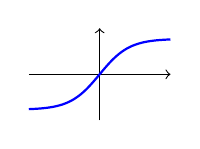
\begin{tikzpicture}[baseline=-0.5ex,scale=0.45]
    \draw[->] (-2,0) -- (2,0);
    \draw[->] (0,-1.3) -- (0,1.3);
    \draw[thick,blue,domain=-2:2,samples=100]
        plot (\x,{1.0*tanh(1.2*\x)});
\end{tikzpicture}
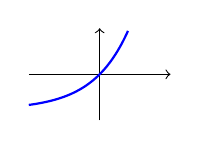
\begin{tikzpicture}[baseline=-0.5ex,scale=0.45]
    \draw[->] (-2,0) -- (2,0);
    \draw[->] (0,-1.3) -- (0,1.3);
    \draw[thick,blue,domain=-2:0.8,samples=100]
        plot (\x,{exp(\x)-1});
\end{tikzpicture}
\\ \hline

$x'<0$ & Decreasing &
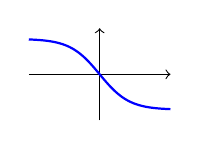
\begin{tikzpicture}[baseline=-0.5ex,scale=0.45]
    \draw[->] (-2,0) -- (2,0);
    \draw[->] (0,-1.3) -- (0,1.3);
    \draw[thick,blue,domain=-2:2,samples=100]
        plot (\x,{-1.0*tanh(1.2*\x)});
\end{tikzpicture}
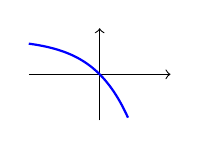
\begin{tikzpicture}[baseline=-0.5ex,scale=0.45]
    \draw[->] (-2,0) -- (2,0);
    \draw[->] (0,-1.3) -- (0,1.3);
    \draw[thick,blue,domain=-2:0.8,samples=100]
        plot (\x,{-exp(\x)+1});
\end{tikzpicture}
\\ \hline

$x'=0$ & Flat &
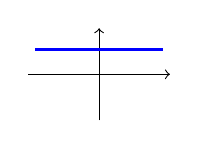
\begin{tikzpicture}[baseline=-0.5ex,scale=0.45]
    \draw[->] (-2,0) -- (2,0);
    \draw[->] (0,-1.3) -- (0,1.3);
    \draw[thick,blue] (-1.8,0.7) -- (1.8,0.7);
\end{tikzpicture}
\end{tabular}
\end{center}
The first of the curves depicted in the shape column for $x'>0$ and $x'<0$ are called \textbf{sigmoid functions} because of their S-shape. Sigmoid functions are common in autonomous equations. Some autonomous equations like 
$$
x' = 4+x^2
$$
satisfy $x'>0$ for all values of $x$. But in general, we should expect a mixture of positive, negative, and zero values of $x'$ as in
$$
x' =(4-x)(2-x)^3.
$$
Consider the set of all real numbers $(-\infty,\infty)$. The sign of $x'$ depends on which subinterval we are in.

% \subsection{Review Family of Solutions}
% Consider the autonomous DE $x'=x-2$. We can solve this DE using separation of variables 
% \begin{align*}
%     \frac{dx}{dt} &= x-2\\
%     \int \frac{dx}{x-2}&=\int dt\\
%     \ln|x-2| &=t+C\\
%     x-2 &= Ce^{t}\\
%     x &= Ce^{t} +2
% \end{align*}
% The general solution can be plotted for several values of $C$ on one graph as a family of solutions. The graph look like exponential functions growing away from $x=2$. If we choose $C=0$, the solution curve is a flat line $x=2$, which happens to be the equilibrium solution. Recall that solution curves are NOT allowed to intersect one another.
% \begin{figure}[H]
%     \centering
% \begin{tikzpicture}[scale=0.9]
% \begin{scope}
%     % Axes
%     \draw[->,thick] (-0.2,0) -- (4.5,0) node[right] {$t$};
%     \draw[->,thick] (0,-1) -- (0,5) node[above] {$x$};
%     % Curves x(t) = C e^{-t}
%     \draw[thick,domain=0:3.5,samples=100] plot (\x,{   1*exp(0.3*\x)+2});
%     \draw[thick,domain=0:3.5,samples=100] plot (\x,{ 0.5*exp(0.3*\x)+2});
%     \draw[thick,domain=0:3.5,samples=100] plot (\x,{-0.5*exp(0.3*\x)+2});
%     \draw[thick,domain=0:3.5,samples=100] plot (\x,{-1.0*exp(0.3*\x)+2});
%     \draw[thick,dashed,domain=0:4,samples=100] plot (\x,2);
%     \node[right] at (4,2) {$x^*=2$};
% \end{scope}
% \end{tikzpicture}\caption{This figure shows the family of solutions to $x'=x-2$. Solutions below $x=2$ are all decreasing. All solutions above $x=2$ are increasing.}
% \end{figure}

\subsection{How to Determine Signs}
Given an autonomous DE
\[
x' = f(x),
\]
we want to determine where $x'$ is positive and where it is negative. Use the following steps:
\begin{enumerate}
    \item Find the equilibria by solving $f(x)=0$.
    \item Mark the equilibria on a number line. These points divide the line into intervals.
    \item Choose one test point from each interval.
    \item Evaluate $f(x)$ at each test point to determine the sign of $x'$ on that interval.
\end{enumerate}
Here is an example.

\begin{example}[1]{
For the DE 
$$
x' = (4-x)(2-x)^3
$$
find the intervals of $x$ on which solution curves are increasing or decreasing.
}
First, set $f(x)=(4-x)(2-x)^3=0$ and solve. 
$$
(4-x)(2-x)^3=0 \implies x^*=2,4.
$$
Next, mark the equilibria on a number line. These points divide the real line into three intervals.

\begin{figure}[H]
    \centering
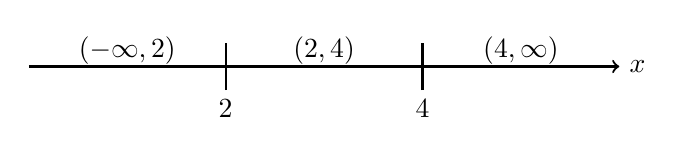
\begin{tikzpicture}[scale=2.5]
\begin{scope}

    \draw[->,thick] (-1,0) -- (2,0) node[right] {$x$}; % line 
    \draw[thick] (-0,-0.12) -- (0,0.12);    % ticks
    \draw[thick] (1.0,-0.12) -- (1.0,0.12);
    \node[below] at (0,-0.12) {$2$};        % tick labels
    \node[below] at (1,-0.12) {$4$};
    \node[below] at (-0.5,0.2) {$(-\infty,2)$};
    \node[below] at (0.5,0.2) {$(2,4)$};
    \node[below] at (1.5,0.2) {$(4,\infty)$};
\end{scope}
\end{tikzpicture}
\end{figure}
On each interval, choose a convenient test point and evaluate $f(x)$ to determine the sign of $x'$.

\[
\begin{array}{c|c|c}
\text{interval} & \text{test point} & f(x) \\
\hline
(-\infty,2) & x=0 & f(0)=(4)(2)^3=32>0 \\
(2,4) & x=3 & f(3)=(1)(-1)^3=-1<0 \\
(4,\infty) & x=5 & f(5)=(-1)(-3)^3=27>0
\end{array}
\]    
Based on the sign, we know 
\[
\boxed{
\text{solutions are increasing on }(-\infty,2)\cup(4,\infty)
\text{ and decreasing on }(2,4).
}
\]
\end{example}

\subsection{Creating Zones}
Recall that the \textit{family of solutions} to the autonomous equation
\[
x' = (4-x)(2-x)^3
\]
consists of all functions that satisfy the DE. The equilibrium solutions
\[
x(t)=2
\qquad \text{and} \qquad
x(t)=4
\]
are part of this family. Since solution curves cannot cross an equilibrium solution, these two equilibria divide the $tx$-plane into three distinct \textit{zones}. If a solution $x(t)$ begins in one zone, then it must remain in that zone for all time.

Furthermore, within each zone, the sign of $x'$ is fixed. Therefore, solutions in each zone must be either increasing or decreasing. The figure below illustrates the three zones.

\begin{figure}[H]
    \centering
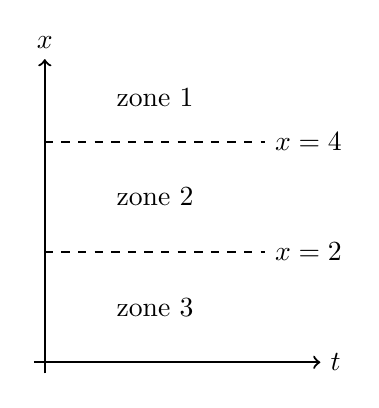
\begin{tikzpicture}[scale=0.7]
\begin{scope}
    % Axes
    \draw[->,thick] (-0.2,0) -- (5,0) node[right] {$t$};
    \draw[->,thick] (0,-0.2) -- (0,5.5) node[above] {$x$};

    % Equilibrium solutions
    \draw[thick,dashed] (0,2) -- (4,2);
    \node[right] at (4,2) {$x=2$};

    \draw[thick,dashed] (0,4) -- (4,4);
    \node[right] at (4,4) {$x=4$};

    % Zones
    \node at (2,4.8) {\text{zone 1}};
    \node at (2,3) {\text{zone 2}};
    \node at (2,1) {\text{zone 3}};
\end{scope}
\end{tikzpicture}
\caption{The equilibrium solutions $x=2$ and $x=4$ split the $tx$-plane into three zones. In each zone, solutions to the autonomous DE are either increasing or decreasing.}
\end{figure}

\subsection{Sketching Solutions}
We are now ready to sketch \textit{qualitative} solution curves for autonomous equations. Here are the steps: 
\begin{enumerate}
    \item Sketch all equilibrium solutions.
    \item Identify each zone as either increasing or decreasing.
    \item Sketch several solution curves in each zone that are consistent with this behavior.
\end{enumerate}

\begin{example}[2]{
Sketch qualitative solution curves for the DE
$$
x' = (4-x)(2-x)^3.
$$
}
Based on Example 1, we know that solutions are increasing in zone 1,
$(4,\infty)$, and zone 3, $(-\infty,2)$, while solutions are decreasing
in zone 2, $(2,4)$. Therefore, in zone 1, sketch curves that rise away
from $x=4$. In zone 2, sketch decreasing curves that approach $x=2$.
In zone 3, sketch increasing curves that approach $x=2$. 
\begin{figure}[H]
\centering
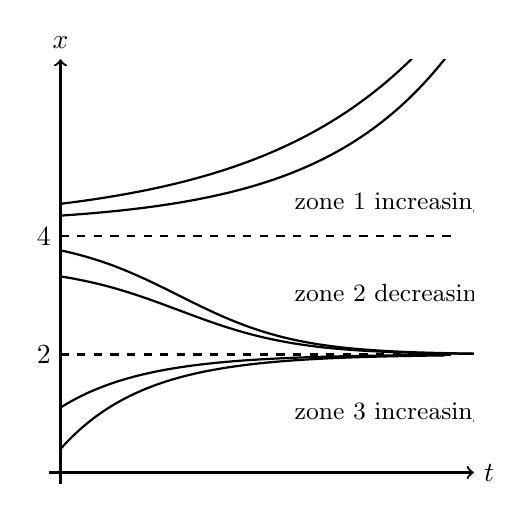
\begin{tikzpicture}[scale=0.75]
    % axes
    \draw[->,thick] (-0.2,0) -- (7.0,0) node[right] {$t$};
    \draw[->,thick] (0,-0.2) -- (0,7) node[above] {$x$};

    % equilibria as horizontal dashed lines
    \draw[dashed,thick] (0,2.0) -- (6.7,2.0);
    \draw[dashed,thick] (0,4.0) -- (6.7,4.0);
    \node[left] at (0,2.0) {$2$};
    \node[left] at (0,4.0) {$4$};
    
    % truncate
    \clip (-0.2,-0.2) rectangle (7,7);

    % solutions approaching x=2 from below
    \draw[thick,domain=0:6.5,samples=200]
        plot (\x,{2.0 - 1.6*exp(-0.7*\x)});
    \draw[thick,domain=0:6.5,samples=200]
        plot (\x,{2.0 - 0.9*exp(-0.7*\x)});

    % solutions approaching x=2 from above (but below 4)
    \draw[thick,domain=-0:7,samples=100] plot (\x,{2+2/(1+exp(\x-2)});
    \draw[thick,domain=-0:7,samples=100] plot (\x,{2+1.5/(1+exp(\x-2)});

    % solutions above 4 increasing away (qualitative growth)
    \draw[thick,domain=0:7.0,samples=200]
        plot (\x,{4.2 + 0.35*exp(0.35*\x)});
    \draw[thick,domain=0:7.0,samples=200]
        plot (\x,{4.2 + 0.15*exp(0.45*\x)});

    % labels
    \node[right] at (3.8,4.55) {\small zone 1 increasing};
    \node[right] at (3.8,3.00) {\small zone 2 decreasing};
    \node[right] at (3.8,1.00) {\small zone 3 increasing};
\end{tikzpicture}
\end{figure}
\end{example}
When we study autonomous DEs, our main goal is often \textit{qualitative}: we want to understand the overall behavior of solutions without finding an exact formula for $x(t)$. It does not matter if our solution curves are slightly inaccurate. 

%-------------------------------------------------------------
\section{Graphical Tools}

\subsection{The $x'$ vs. $x$ Graph}

For an autonomous DE
\[
    x'=f(x),
\]
the \textbf{$x'$ versus $x$ graph} is simply the graph of $f(x)$, with $x$
on the horizontal axis and $x'$ on the vertical axis. The main advantage of the $x'$ versus $x$ graph is that it immediately reveals where $x'$ is positive or negative. If the curve $f(x)$ is under the $x$-axis, then $x'$ is negative. If the curve $f(x)$ is above the $x$-axis, then $x'$ is positive. Think of this as an alternative to using test points. 


\begin{example}[3]{
Sketch the $x'$ versus $x$ graph for 
\[
    x'=x(1-x).
\]
Then indicate the intervals on which solution curves are increasing or decreasing.
}
Sketch $f(x)=x(1-x)=-x^2+x$. This is a downward-opening parabola with intercepts at $x=0$ and $x=1$. 
\begin{figure}[H]
    \centering
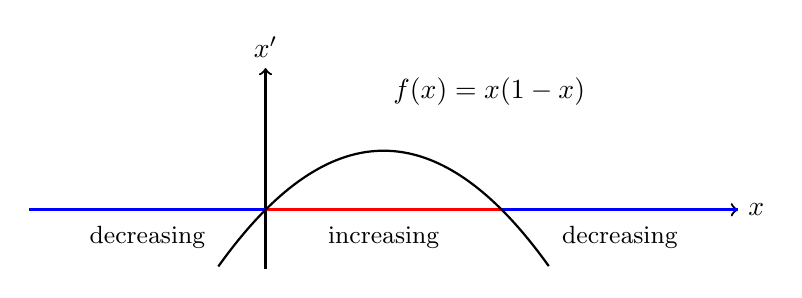
\begin{tikzpicture}[scale=3]
\begin{scope}
    % Axes
    \draw[->,thick] (-1,0) -- (2,0) node[right] {$x$};
    \draw[->,thick] (0,-.25) -- (0,0.6) node[above] {$x'$};
    \draw[very thick,blue] (-1,0) -- (0,0);
    \draw[very thick,blue] (1,0) -- (2,0);
    \draw[very thick,red] (0,0) -- (1,0);
    % Curves x(t) = C e^{-t}
    \draw[thick,domain=-0.2:1.2,samples=100] plot (\x,{ \x*(1-\x)});
    \node[right] at (0.5,0.5) {$f(x)=x(1-x)$};

    \node[below] at (-0.5,-0.03) {\small decreasing};
    \node[below] at (0.5,-0.03) {\small increasing};
    \node[below] at (1.5,-0.03) {\small decreasing};
\end{scope}
\end{tikzpicture}
\end{figure}
Graphically, we see that $f(x)=x(1-x)$ is \textit{below} the $x$-axis on $(-\infty,0)$ and on $(1,\infty)$. The curve is \textit{above} the $x$-axis on $(0,1)$. Knowing that $x'=f(x)$, we can conclude that 
\[
\boxed{
\text{solutions are decreasing on }(-\infty,0)\cup(1,\infty)
\text{ and increasing on }(0,1).
}
\]
\end{example}

\subsection{The Phase Line}

The \textbf{phase line} is a one-dimensional diagram that shows the
direction in which solutions move along the $x$-axis. For an autonomous DE $x'=f(x)$, the phase line is constructed as follows:
\begin{enumerate}
    \item Draw a number line for $x$.
    \item Find all equilibria and label them on the number line.
    \item On each interval separated by the equilibria,
    \begin{itemize}
        \item draw a right arrow if $x'>0$,
        \item draw a left arrow if $x'<0$.
    \end{itemize}
\end{enumerate}

\begin{example}[4]{
Sketch the phase line for
\[
    x'=x(1-x).
\]
}
We already know where $x'$ is positive and negative from the $x'$ versus
$x$ graph. The corresponding phase line is shown below. A \textbf{left arrow} is drawn on the intervals $(-\infty,0)$ and $(1,\infty)$ because $x'$ is negative. A \textbf{right arrow} is drawn on the interval $(0,1)$ because $x'>0$. 
\begin{figure}[H]
    \centering
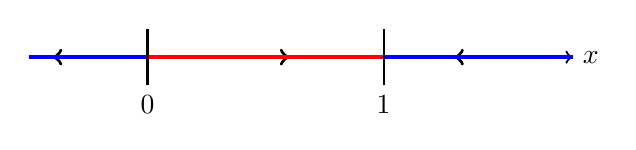
\begin{tikzpicture}[scale=3]
\begin{scope}
    
    % arrows: x<0 left
    \draw[->,very thick] (-0.3,0) -- (-0.4,0);
    % arrows: 0<x<1 right
    \draw[->,very thick] (0.4,0) -- (.6,0);
    % arrows: x>1 left
    \draw[->,very thick] (1.4,0) -- (1.3,0);
    
    % Axes
    \draw[->,thick] (-0.5,0) -- (1.8,0) node[right] {$x$};
    \draw[very thick,blue] (-0.5,0) -- (0,0);
    \draw[very thick,blue] (1,0) -- (1.8,0);
    \draw[very thick,red] (0,0) -- (1,0);
        % ticks at equilibria
    \draw[thick] (-0,-0.12) -- (0,0.12);
    \draw[thick] (1.0,-0.12) -- (1.0,0.12);
    \node[below] at (0,-0.12) {$0$};
    \node[below] at (1,-0.12) {$1$};
\end{scope}
\end{tikzpicture}
\end{figure}

\end{example}

\subsection{Solution Curves}
The main payoff of our qualitative analysis is that we can sketch solution
curves in the $tx$-plane without explicitly solving the differential
equation. The textbook refers to these graphs as \textbf{time series plots}. The solution curves tell us the limiting behavior of solution curves depending on the value of the initial condition. 

\begin{example}[5]{
Sketch several qualitative solution curves for
$$
x' = x(1-x)
$$
on the $tx$-plane. Then state the limiting behavior of the particular solution satisfying the initial condition
$$
x(0)=0.5.
$$
}
We begin by plotting the equilibrium solutions $x^*= 0,1$. In zone 1 $(1,\infty)$, we draw decreasing curves that flatten out towards $x^*=1$ because $x'<0$. In zone 2 $(0,1)$, we draw rising sigmoid curves that flatten out toward $x^*=1$ because $x'>0$. Lastly, in zone 3 $(-\infty,0)$, we draw decreasing curves because $x'<0$.  

\begin{figure}[H]
\centering
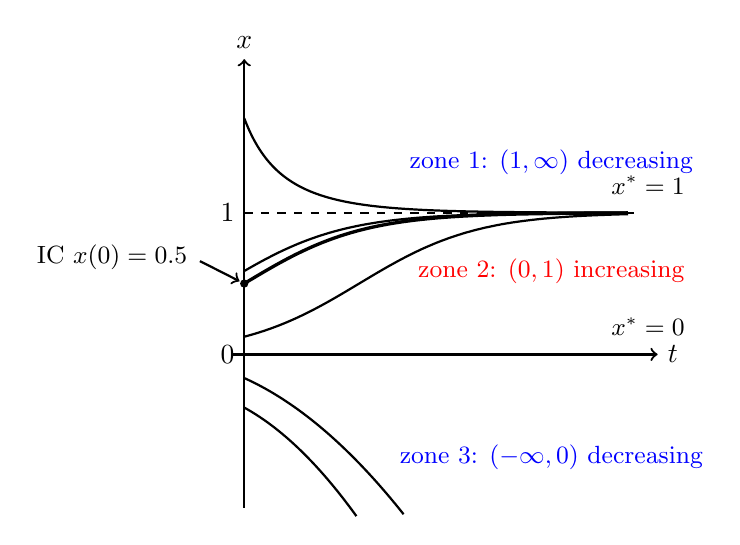
\begin{tikzpicture}[scale=0.75]
    % axes
    \draw[->,thick] (-0.2,0) -- (7,0) node[right] {$t$};
    \draw[->,thick] (0,-2.6) -- (0,5) node[above] {$x$};
    % equilibria: x=0 and x=1
    \draw[dashed,thick] (0,0) -- (6.6,0);
    \node[left] at (0,0) {$0$};
    \draw[dashed,thick] (0,2.4) -- (6.6,2.4);
    \node[left] at (0,2.4) {$1$};
    % (i) 0 < x0 < 1 : increasing to 1
    \draw[thick,domain=0:6.5,samples=200]
        plot (\x,{2.4*(1/(1 + 7*exp(-\x)))});
    % \draw[thick,domain=0:6.5,samples=200]
    %     plot (\x,{2.4*(1/(1 + 2*exp(-\x)))});
    \draw[very thick,domain=0:6.5,samples=200]
    plot (\x,{2.4*(1/(1 + exp(-\x)))});
    \draw[thick,domain=0:6.5,samples=200]
        plot (\x,{2.4*(1/(1 + 0.7*exp(-\x)))});

    % (ii) x0 > 1 : decreasing to 1  (A<0)
    \draw[thick,domain=0:6.5,samples=200]
        plot (\x,{2.4*(1/(1 - 0.4*exp(-\x)))});

    % (iii) x0 < 0 : decreasing downward (qualitative sketch)
    % Use a simple curve that drops faster over time (not the exact formula).
    \draw[thick,domain=0:2.7,samples=120]
        plot (\x,{-0.4 - 0.45*\x - 0.15*\x*\x});
    \draw[thick,domain=0:1.9,samples=120]
        plot (\x,{-0.9 - 0.55*\x - 0.22*\x*\x});

    % labels near the right side
    \node[above right] at (6.05,2.55) {\small  $x^*=1$};
    \node[above right] at (6.05,0.15) {\small $x^*=0$};

    % optional zone notes (remove if you want it cleaner)
    \node[blue] at (5.2,3.25) {\small zone 1: $(1,\infty)$ decreasing};
    \node[red] at  (5.2,1.4) {\small zone 2: $(0,1)$ increasing };
    \node[blue] at (5.2,-1.75) {\small zone 3: $(-\infty,0)$ decreasing};

    % Initial condition x(0)=0.5
    \fill (0,1.2) circle (2pt);
    
    % Initial condition label
    \node[left] at (-0.8,1.65) {\small IC $x(0)=0.5$};
    \draw[->,thick]
        (-0.75,1.58) -- (-0.08,1.24);
        
\end{tikzpicture}
\end{figure}
Since the initial value of $x$ is $x_0=0.5$ is in the interval $(0,1)$, we know that the solution curve lives in zone 2. Therefore, we can conclude that 
$$
\boxed{
\lim_{t\to\infty} x(t)= 1.
}
$$
\end{example}


%-------------------------------------------------------------
\section{Stability}
I'll avoid stating the real definition of stability because I want to avoid unnecessary confusion. A more detailed explanation of stability can be found in the textbook.

\subsection{Informal Definition}
\textbf{Stability} describes how solutions behave near an equilibrium $x^*$. If nearby solutions move toward $x^*$, the equilibrium is \textbf{stable}.  If nearby solutions move away from $x^*$, the equilibrium is \textbf{unstable}.

\subsection{Phase Line and Stability}

We will use the phase line to classify the type of stability of the equilibria. Each equilibrium point $x^*$ on the phase line has an arrow to its left and to its right. The direction of the two arrows defines the classification of $x^*$. There are 3 classifications:
\begin{itemize}
    \item \textbf{Stable:} both arrows point \emph{toward} $x^*$.
    \[
    \longrightarrow\ \CIRCLE \longleftarrow
    \]
    \item \textbf{Unstable:} at least one arrow points \emph{away from} $x^*$.
    \[
    \longleftarrow\ \Circle \longrightarrow
    \]
    \item \textbf{Semistable:} one arrow point in and the other points out.
    \[
    \longrightarrow\ \LEFTcircle \longrightarrow
    \qquad\text{or}\qquad
    \longleftarrow\ \RIGHTcircle  \longleftarrow
    \]
\end{itemize}
Semistable equilibria are technically unstable, but if you are asked to distinguish between stable, unstable, and semistable, then you should do so. 

\begin{example}[6]{
Consider the DE 
$$x' = x(1-x).$$
State all equilibria and their stability (stable, unstable, semistable). }

We have already found the equilibria $x^*=0,1$ and drawn the phase line. Since both arrows to either side of $x^*=0$ point \textit{away} from it, $x^*=0$ is \textbf{unstable}. Since both arrows to either side of $x^*=1$ point \textit{toward} it, $x^*=1$ is \textbf{stable}.

\begin{figure}[H]
    \centering
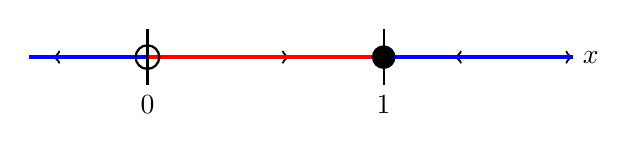
\begin{tikzpicture}[scale=3]
\begin{scope}
    % arrows: x<0 left
    \draw[->,thick] (-0.3,0) -- (-0.4,0);
    % arrows: 0<x<1 right
    \draw[->,thick] (0.4,0) -- (.6,0);
    % arrows: x>1 left
    \draw[->,thick] (1.4,0) -- (1.3,0);
    % Axes
    \draw[->,thick] (-0.5,0) -- (1.8,0) node[right] {$x$};
    \draw[very thick,blue] (-0.5,0) -- (0,0);
    \draw[very thick,blue] (1,0) -- (1.8,0);
    \draw[very thick,red] (0,0) -- (1,0);
        % ticks at equilibria
    \draw[thick] (-0,-0.12) -- (0,0.12);
    \draw[thick] (1.0,-0.12) -- (1.0,0.12);
    \node[below] at (0,-0.12) {$0$};
    \node[below] at (1,-0.12) {$1$};
        \fill (1,0) circle (0.05);
        \draw[thick] (0,0) circle (0.05);
\end{scope}
\end{tikzpicture}
\end{figure}
\end{example}

\subsection{Analytic Stability Criterion}
There is a calculus-based test that tells us the stability of an equilibrium point. Let $x^*$ be an equilibrium, so $f(x^*)=0$.
If $f$ is differentiable at $x^*$, then:
\begin{itemize}
    \item If $f'(x^*)<0$, then $x^*$ is \textbf{stable}.
    \item If $f'(x^*)>0$, then $x^*$ is \textbf{unstable}.
    \item If $f'(x^*)=0$, the test is inconclusive. 
\end{itemize}
For example, $x'=x(1-x)=x-x^2$ has a stable equilibrium at $x^*=1$. We calculate 
\begin{align*}    
f'(x) &= 1-2x\\
f'(1)&=-1<0.
\end{align*}
Since $f'(1)$ is negative, the test confirms that $x^*=1$ is stable. Meanwhile, $f'(0)=1$ is positive so $x^*=0$ is unstable according to the analytic stability tests. 

Since we can use the phase line to determine stability, this tool isn't necessary. You will not be tested on this. The homework does not require you to use this test.  That said, it is nice to check your work. You can read more about this in your textbook. 

%-------------------------------------------------------------
\section{Sketching Polynomials}


A part of the homework assignment consists of sketching $x'$ versus $x$ graphs for
$$
x'=f(x)
$$
where $f(x)$ is a polynomial. Although sketching 3rd degree or higher polynomials is a challenge, we do not need to be precise. Begin by finding the $x$-intercepts. Then use information about the sign of $f(x)$ in between the intercepts to draw a plausible shape for the polynomial. We'll do a couple of examples.


\begin{example}[7]{
Sketch the $x'$ versus $x$ graph for 
$$x'=(4-x)(2-x)^3.$$
}
We have already studied this equation in Example 1. This is what we found:
\[
\begin{array}{c|c|c}
\text{interval} & \text{test point} & \text{sign of }f(x) \\
\hline
(-\infty,2) & x=0 & f(0)=(4)(2)^3=32>0 \\
(2,4) & x=3 & f(3)=(1)(-1)^3=-1<0 \\
(4,\infty) & x=5 & f(5)=(-1)(-3)^3=27>0
\end{array}
\]   
Begin by marking the two intercepts $x=2,4$. On the interval $x\in(-\infty,2)$, $f(x)$ should be above the $x$-axis. Then on the interval $x\in(2,4)$, $f(x)$ should be below the $x$-axis. Finally, on the last interval, $f(x)$ should be above the $x$-axis.

\begin{figure}[H]
\centering
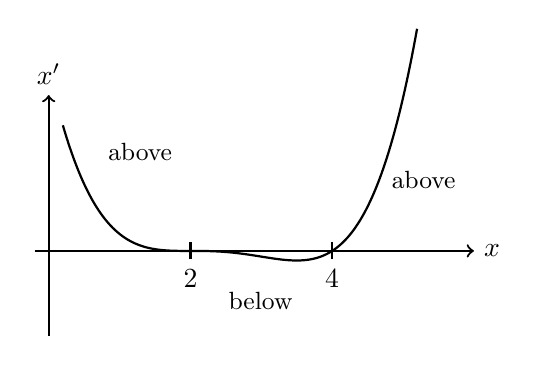
\begin{tikzpicture}[scale=0.90]
    % axes
    \draw[->,thick] (-0.2,0) -- (6.0,0) node[right] {$x$};
    \draw[->,thick] (0,-1.2) -- (0,2.2) node[above] {$x'$};
    % labels for equilibria on x-axis
    \draw[thick] (2,-0.12) -- (2,0.12);
    \draw[thick] (4,-0.12) -- (4,0.12);
    \node[below] at (2,-0.12) {$2$};
    \node[below] at (4,-0.12) {$4$};

    % a qualitative sketch of f(x):
    % above axis for x<2, crosses at 2, below on (2,4), crosses at 4, above after 4
    \draw[thick,domain=0.2:5.2,samples=200]
        plot (\x,{0.08*(4-\x)*((2-\x)^3)});
    \node[right] at (0.7,1.4) {\small above};
    \node[right] at (2.4,-0.7) {\small below};
    \node[right] at (4.7,1.0) {\small above};
\end{tikzpicture}
\end{figure}
\end{example}

\begin{example}[8]{
Sketch the $x'$ versus $x$ graph for 
$$x'=-kx+d,$$
where $k$ and $d$ are positive constants.
}
First, find the equilibrium: 
$$
    -kx+d=0\implies x^* = d/k.
$$
Since both $k$ and $d$ are positive, we know $x^*=d/k>0$. The $y$-intercept is $f(0)=d$ is also positive. Draw a straight line connecting the $y$-intercept and the $x$-intercept. 

\begin{figure}[H]
\centering
\begin{tikzpicture}[scale=0.90]
    % axes
    \draw[->,thick] (-0.2,0) -- (6.0,0) node[right] {$x$};
    \draw[->,thick] (0,-1.2) -- (0,2.2) node[above] {$x'$};
    % labels for equilibria on x-axis
    \draw[thick] (3,-0.12) -- (3,0.12);
    \node[below] at (3,-0.12) {$x=\tfrac{d}{k}$};
    \draw[thick] (-0.12,1.5) -- (0.12,1.5);
    \node[left] at (-0.14,1.5) {$x'=d$};

    % a qualitative sketch of f(x):
    \draw[thick,domain=-0.2:5.2,samples=200] plot (\x,{-0.5*\x+1.5});
    
\end{tikzpicture}
\end{figure}
\end{example}


% Consider the autonomous DE
% \[
% x' = (4-x)(2-x)^3.
% \]
% \begin{itemize}
%     \item Find the equilibria,
%     \item Sketch the phase line,
%     \item Classify the stability of the equilibria,
%     \item Plot the growth rate $f(x)$ (an $x'$ vs.\ $x$ graph),
%     \item Sketch key time series curves in the $tx$-plane.
% \end{itemize}


% \subsection*{Step 1: Equilibria}
% Equilibria occur when $x'=0$, i.e.\ when $f(x)=0$:
% \[
% (4-x)(2-x)^3=0
% \quad\Longrightarrow\quad
% x^*=2,\ 4.
% \]
% Note that $x=2$ is a \emph{triple root} (multiplicity $3$), while $x=4$ is a simple root.

% \subsection*{Step 2: Sign of $x'$ on intervals}
% We determine the sign of $f(x)$ on the intervals $(-\infty,2)$, $(2,4)$, and $(4,\infty)$ by test points. Choose convenient integers to plug into $f(x)$ for each subinterval.
% \[
% \begin{array}{c|c|c}
% \text{interval} & \text{test point} & f(x) \\
% \hline
% (-\infty,2) & x=0 & f(0)=(4)(2)^3=32>0 \\
% (2,4) & x=3 & f(3)=(1)(-1)^3=-1<0 \\
% (4,\infty) & x=5 & f(5)=(-1)(-3)^3=27>0
% \end{array}
% \]

% \subsection*{Step 3: Phase line and stability}
% From the sign information:
% \begin{itemize}
%     \item $x^*=2$: arrows point \emph{toward} $2$ from both sides, so $x^*=2$ is \textbf{stable}.
%     \item $x^*=4$: arrows point \emph{away} from $4$ from both sides, so $x^*=4$ is \textbf{unstable}.
% \end{itemize}

% \begin{figure}[H]
% \centering
% \begin{tikzpicture}[scale=2.6]
%     % number line
%     \draw[->,thick] (1,0) -- (5,0) node[right] {$x$};

%     % arrows based on sign: (+) then (-) then (+)
%     % (-inf,2): right
%     \draw[->,thick] (0.8,0) -- (1.3,0);
%     % (2,4): left
%     \draw[->,thick] (3.2,0) -- (2.7,0);
%     % (4,inf): right
%     \draw[->,thick] (4.3,0) -- (4.75,0);

%     % ticks
%     \draw[thick] (2,-0.12) -- (2,0.12);
%     \draw[thick] (4,-0.12) -- (4,0.12);

%     % equilibrium markers: stable at 2 (filled), unstable at 4 (open)
%     \fill (2,0) circle (0.06);
%     \draw[thick] (4,0) circle (0.06);

%     % labels
%     \node[below] at (2,-0.12) {$2$};
%     \node[below] at (4,-0.12) {$4$};
%     \node[above] at (2,0.18) {\small stable};
%     \node[above] at (4,0.18) {\small unstable};
% \end{tikzpicture}
% \caption{Phase line for $x'=(4-x)(2-x)^3$.}
% \label{fig:phaseline_ex}
% \end{figure}

% \subsection*{Step 4: $x'$ versus $x$ graph (growth rate plot)}
% A rough sketch of $f(x)$ is enough for analysis:
% \begin{itemize}
%     \item $f(x)=0$ at $x=2$ and $x=4$.
%     \item $f(x)>0$ for $x<2$.
%     \item $f(x)<0$ for $2<x<4$.
%     \item $f(x)>0$ for $x>4$.
% \end{itemize}
% \begin{figure}[H]
% \centering
% \begin{tikzpicture}[scale=1.00]
%     % axes
%     \draw[->,thick] (-0.2,0) -- (6.0,0) node[right] {$x$};
%     \draw[->,thick] (0,-1.2) -- (0,2.2) node[above] {$x'$};
%     % labels for equilibria on x-axis
%     \draw[thick] (2,-0.12) -- (2,0.12);
%     \draw[thick] (4,-0.12) -- (4,0.12);
%     \node[below] at (2,-0.12) {$2$};
%     \node[below] at (4,-0.12) {$4$};

%     % a qualitative sketch of f(x):
%     % above axis for x<2, crosses at 2, below on (2,4), crosses at 4, above after 4
%     \draw[thick,domain=0.2:5.2,samples=200]
%         plot (\x,{0.08*(4-\x)*((2-\x)^3)});

%     \node[right] at (3.7,1.6) {\small $x'=f(x)$};
% \end{tikzpicture}
% \caption{$x'$ vs.\ $x$ graph for $f(x)=(4-x)(2-x)^3$ (qualitative).}
% \label{fig:fxplot_ex}
% \end{figure}

% \subsection*{Step 5: Time series sketch in the $tx$-plane}
% Now we sketch solution curves $x=x(t)$ using the phase line:
% \begin{itemize}
%     \item If $x_0<2$, then $x'>0$, so solutions \textbf{increase} and approach $x=2$.
%     \item If $2<x_0<4$, then $x'<0$, so solutions \textbf{decrease} and approach $x=2$.
%     \item If $x_0>4$, then $x'>0$, so solutions \textbf{increase away from} $x=4$ and grow without bound.
% \end{itemize}

% \begin{figure}[H]
% \centering
% \begin{tikzpicture}[scale=0.95]
%     % axes
%     \draw[->,thick] (-0.2,0) -- (7.0,0) node[right] {$t$};
%     \draw[->,thick] (0,-0.2) -- (0,7.2) node[above] {$x$};

%     % equilibria as horizontal dashed lines
%     \draw[dashed,thick] (0,2.2) -- (6.7,2.2);
%     \draw[dashed,thick] (0,4.2) -- (6.7,4.2);
%     \node[left] at (0,2.2) {$2$};
%     \node[left] at (0,4.2) {$4$};

%     % solutions approaching x=2 from below
%     \draw[thick,domain=0:6.5,samples=200]
%         plot (\x,{2.2 - 1.6*exp(-0.7*\x)});
%     \draw[thick,domain=0:6.5,samples=200]
%         plot (\x,{2.2 - 0.9*exp(-0.7*\x)});

%     % solutions approaching x=2 from above (but below 4)
%     \draw[thick,domain=0:6.5,samples=200]
%         plot (\x,{2.2 + 1.4*exp(-0.7*\x)});
%     \draw[thick,domain=0:6.5,samples=200]
%         plot (\x,{2.2 + 0.7*exp(-0.7*\x)});

%     % solutions above 4 increasing away (qualitative growth)
%     \draw[thick,domain=0:6.2,samples=200]
%         plot (\x,{4.2 + 0.35*exp(0.35*\x)});
%     \draw[thick,domain=0:5.6,samples=200]
%         plot (\x,{4.2 + 0.15*exp(0.45*\x)});

%     % labels
%     \node[right] at (5.4,2.55) {\small approach $x=2$};
%     \node[right] at (5.2,4.55) {\small $x=4$ unstable};
% \end{tikzpicture}
% \caption{Time series sketch for $x'=(4-x)(2-x)^3$. Solutions in $(2,4)$ and below $2$ approach the stable equilibrium $x=2$. Solutions above $4$ move upward away from $x=4$.}
% \label{fig:timeseries_ex}
% \end{figure}

\end{document}
